\testfile{pgfplotstest.reverseaxis.tex}
{
	\pgfplotsset{compat=newest}

	\testsection{x dir=reverse}
	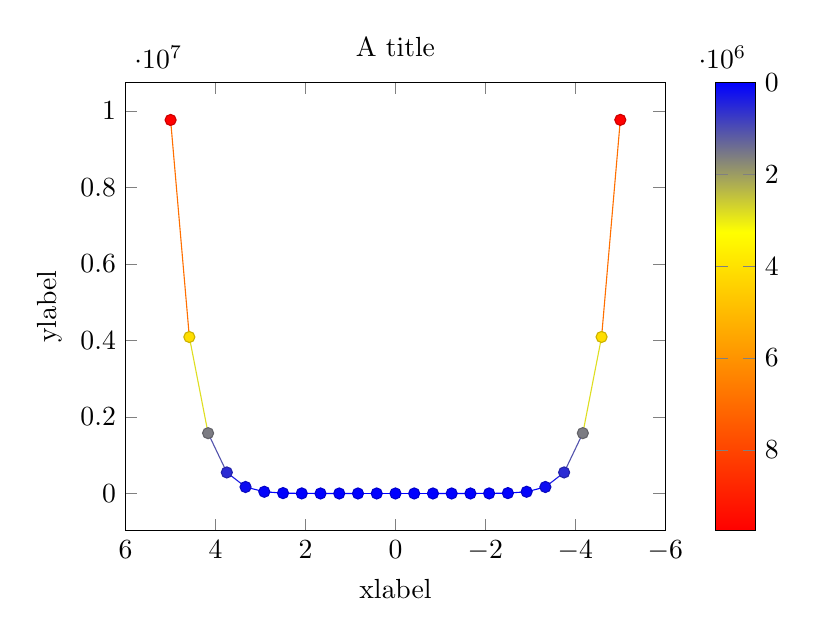
\begin{tikzpicture}
		\begin{axis}[
			x dir=reverse,
			title=A title,
			xlabel=xlabel,
			ylabel=ylabel,
			colorbar,
			clip=false,
			colorbar style={y dir=reverse,clip=false},
		]
		\addplot+[mesh,scatter] {x^10};
		\end{axis}
	\end{tikzpicture}

	\testsection{x dir=reverse,axis lines=left}
	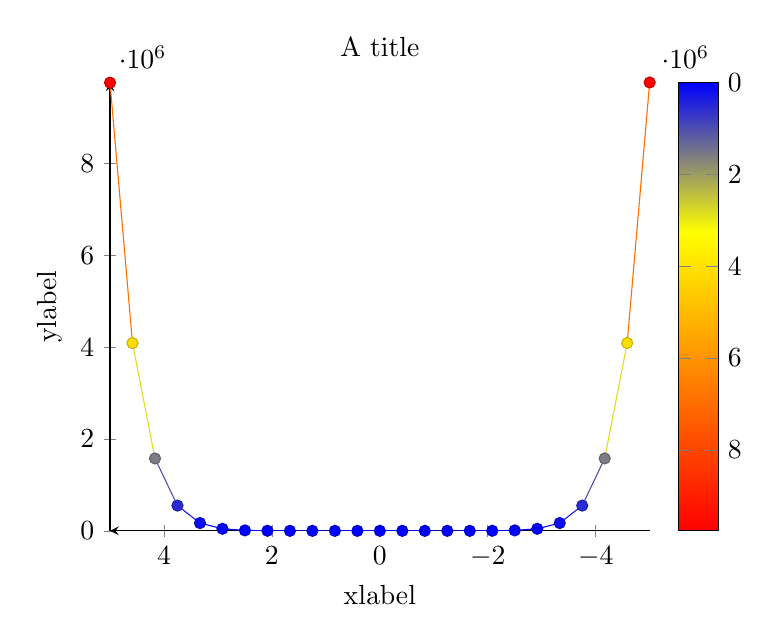
\begin{tikzpicture}
		\begin{axis}[
			axis lines=left,
			x dir=reverse,
			title=A title,
			xlabel=xlabel,
			ylabel=ylabel,
			colorbar,
			colorbar style={y dir=reverse},
		]
		\addplot+[mesh,scatter] {x^10};
		\end{axis}
	\end{tikzpicture}
	
	\testsection{x dir=reverse,axis lines=center}
	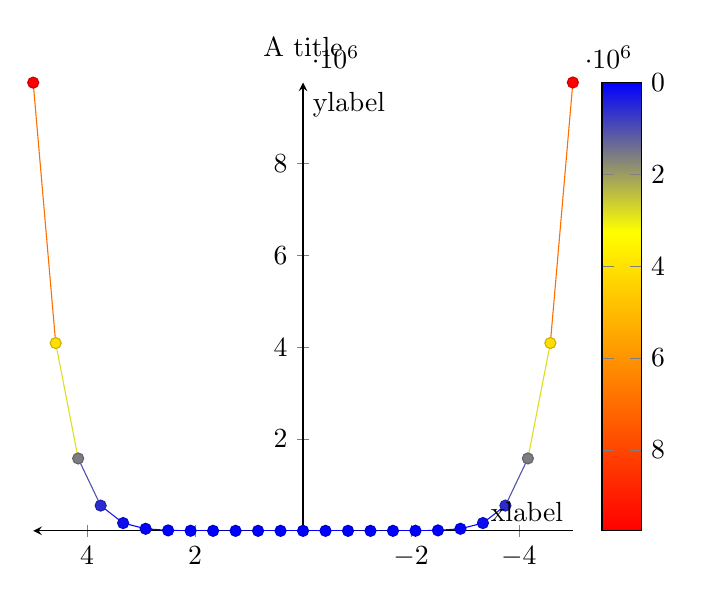
\begin{tikzpicture}
		\begin{axis}[
			axis lines=center,
			x dir=reverse,
			title=A title,
			xlabel=xlabel,
			ylabel=ylabel,
			colorbar,
			colorbar style={y dir=reverse},
		]
		\addplot+[mesh,scatter] {x^10};
		\end{axis}
	\end{tikzpicture}

	\testsection{x dir=reverse,axis lines=right}
	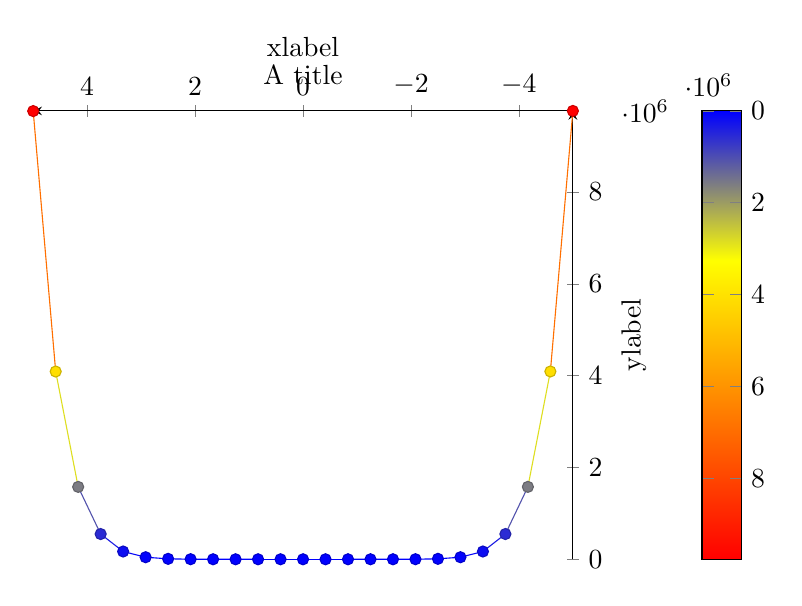
\begin{tikzpicture}
		\begin{axis}[
			axis lines=right,
			x dir=reverse,
			title=A title,
			xlabel=xlabel,
			ylabel=ylabel,
			colorbar,
			colorbar style={y dir=reverse},
		]
		\addplot+[mesh,scatter] {x^10};
		\end{axis}
	\end{tikzpicture}
}
